\documentclass{article}
\usepackage{graphicx}
\begin{document}
Robotic SLAM 
\section{Introduction}
Terms 

\begin{itemize}
    \item State estimation - find out the pose 
    \item Localisation - pose w.r.to landmark or map
    \item Mapping 
   \item navigation and motion planning - a star, wave front dijkstra 
\end{itemize}

\subsection{What is SLAM}
    Computing robot's poses and the map of the environment at the 
    same time.
\textbf{Localisation} : estimating robots location\\ 
\textbf{Mapping}      : building a MAP\\

\textbf{Given}

\begin{itemize}
    \item Robots control inputs   $$u_{1:T} = \{u_1,u_2,u_3....u_T\}$$
    \item Observations $$z_{1:T} = \{z_1,z_2,z_3,...,z_T\}$$
\end{itemize}

\textbf{Wanted}
\begin{itemize}
    \item Map of the environment $$m$$
    \item path of the Robot $$x_{0:T} = \{x_0,x_1,x_2,...,x_T\}$$
\end{itemize}

Using the robots control inputs we can predict the position of the robot.
From the observations $z_{1:T}$, we can calculate the position of the robot. 
Both the steps have some error associcated with it . Lets call the first
one the model noise and second one the sensor noise. So we have to associate 
a probability with both of them. The error accumulates over time(even if the
error in individual measurements is really small)\\

So in the probalistic terms our problem minimises to 
$$p(x_{0:T},m|z_{1:T},u_{1:T})$$


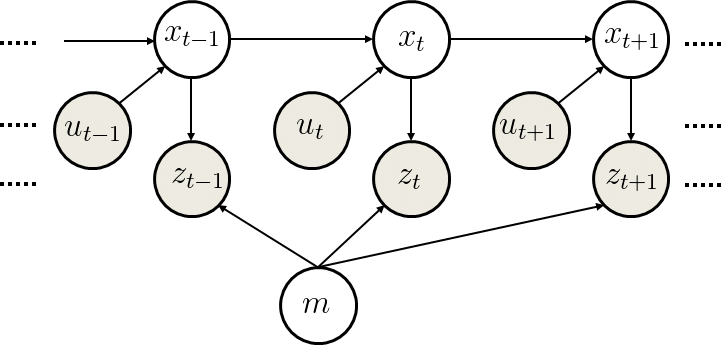
\includegraphics[width = \linewidth]{graphical_model.png}
\subsection{Full Slam vs online SLAM}
    \begin{itemize}
        \item Full SLAM estimates the entire path $$p(x_{0:T},m|z_{1:T},u_{1:T})$$
        \item Online SLAM estimates only the most recent pose $$p(x_{t},m|z_{1:T},u_{1:T})$$
    \end{itemize}
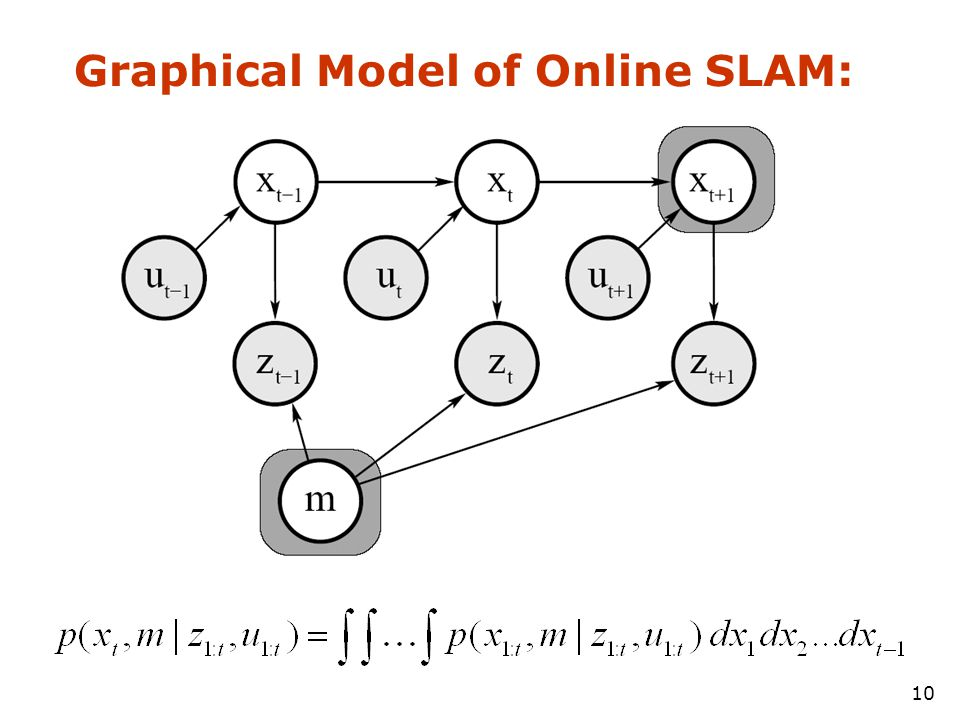
\includegraphics[width = \linewidth]{online_SLAM.jpg}
\end{document}
